\documentclass[a4paper, 10pt]{article}
\usepackage[T1]{fontenc}
\usepackage[utf8]{inputenc}
\usepackage[slovene]{babel}
\usepackage{lmodern}
\usepackage{amsmath}
\usepackage{leftidx}
%\usepackage[style=numeric]{biblatex}
\usepackage{amssymb}
\usepackage{amsthm}
\usepackage{amsfonts}
\usepackage{graphicx}
\usepackage{wrapfig}
\usepackage{amsthm}
\usepackage{mathrsfs}
\usepackage{mathtools}
\usepackage{url}
\usepackage{subfigure}
\usepackage{multirow}
\usepackage{lipsum}
\usepackage{wrapfig}
\usepackage{tikz}
\usepackage[format=plain, font=small, labelfont=bf, textfont=it, justification=centerlast]{caption}
\usepackage{booktabs}
\usepackage{siunitx}

%\newtheorem{izr}{Izrek}
%\newtheorem{posl}{Posledica}[izr]

%\newcounter{defcount}
%\newcounter{opombe}
%\newcounter{zgledcount}

%\newenvironment{opomba}{\begin{flushleft}\stepcounter{opombe}\textbf{Opomba \arabic{opombe}:}}{\hfill\end{flushleft}}
%\setlength{\parindent}{0mm}

%\newenvironment{zgled}{\begin{flushleft}\stepcounter{zgledcount}\textbf{Zgled \arabic{zgledcount}:}}{\hfill\end{flushleft}}
%\setlength{\parindent}{0mm}

%\newenvironment{definicija}{\begin{flushleft}\stepcounter{defcount}\textbf{Definicija \arabic{defcount}:}}{\hfill\end{flushleft}}
%\setlength{\parindent}{0mm}

\newcommand{\naslov}[1]{\textit{#1}}
\newcommand{\abs}[1]{\ensuremath{\lvert #1 \rvert}}
\newcommand{\mth}[1]{\ensuremath{\mathbb{#1}}}
\newcommand{\R}{\mth{R}}
\newcommand{\Z}{\mth{Z}}
\newcommand{\Zp}{\mth{Z}^{+}}
\newcommand{\N}{\mth{N}}
\newcommand{\No}{\mth{N}_0}
\newcommand{\C}{\mth{C}}
\newcommand{\Qu}{\mth{Q}_u}
\newcommand{\pojem}[1]{\emph{#1}}
\newcommand{\con}{\ensuremath{\mathscr{C}}}
\newcommand{\padex}[2]{\ensuremath{{#1}^{\underline{#2}}}}
\newcommand{\rastx}[2]{\ensuremath{{#1}^{\bar{#2}}}}
\newcommand{\map}[3]{\ensuremath{{#1}: {#2} \rightarrow {#3}}}
\newcommand{\pra}[3]{{#1}{\ast}({#2}) = {#3}}

\title{Projektna naloga pri Statistiki}
\date{17.7.2022}
\author{Jimmy Zakeršnik}
%===============================================================================
\begin{document}
	\maketitle
	\thispagestyle{empty}
	\newpage
	\begin{abstract}
		V tej nalogi pri predmetu Statistika, so obravnavane tri naloge, vsaka v svojem lastnem poglavju. V prvem poglavju se obravnava dohodke družin mesta Kibergrad s pomočjo enostavnega slučajnega vzorčenja, škatel z brki ter analize s tipom družine pojasnjene variance dohodka. V drugem poglavju se s pomočjo Rayleighove porazdelitve $Rayleigh(\theta)$ obravnavajo izmerjene dolžine kromatina. Za parameter $\theta$ se določita cenilki po metodi največjega verjetja ter po metodi momentov. Obe cenilki sta tudi primerjani glede na asimptotsko $MSE$ in nepristranskost, nato pa se tudi izračuna njuno numerično vrednost na podlagi priloženih podatkov in primerja prileganje pripadajočih verjetij s histogrami podatkov. V zadnjem poglavju, se obravnavata regresijska modela $A$ ter $B$. Model $A$ je zavrnjen znotraj $B$ pri stopnji tveganja $0{,}05$, sprejet pa pri stopnji tveganja $0{,}01$. S pomočjo Akaikejeve informacije se pokaže, da je model $B$ bolj optimalen za obravnavo povprečnih mesečnih temperatur, kot pa model $A$.
	\end{abstract}
	\newpage
	\tableofcontents
	\listoffigures
	\listoftables
	\newpage
	\section{Kibergrad}\label{sect: Kibergrad}
	Priložena datoteka \textit{Kibergrad.csv}, ki vsebuje podatke o dani populaciji (prebivalci mesta Kibergrad), je bila odprta v programu LibreOffice Calc. S pomočjo vgrajenega orodja so nato, bili zbrani vzorci velikosti $500$ po postopku enostavnega vzorčenja. V priloženi datoteki \textit{Kibergradwork.ods} so na prvi strani izpisani vsi podatki ter vseh pet pridobljenih vzorcev, na drugi strani je posebej obravnavan prvi vzorec v smislu kvartilov in extremnih vrednosti, na tretji strani pa se na enak način obravnavajo vsi vzorci glede na dohodek družin tipa $1$. Obe primerjavi sta dodatno podprti s pomočjo škatel z brki in na koncu sta izračunani še s tipi pojasnjena varianca in nepojasnjena varianca dohodkov. Pri tem je v veliko pomoč programski jezik \textbf{R}.
	
	\subsection{Primerjava dohodkov med tipi družin prvega vzorca} \label{subsect: 1A}
	Poglejmo si najprej prvi vzorec in primerjajmo dohodke družin glede na tip družine. Za pravilno delovanje vsake od skript, ki so omenjene v tej nalogi, je ključno to, da je delovno okolje pravilno nastavljeno na mapo \textit{Podatki\_in\_skripte}. Za delovno okolje torej nastavimo to mapo ter odpremo in poženemo skripto \textit{Kibergrad\_a.R}, napisano v jeziku $\textbf{R}$. Ob pogonu se v konzoli izpišejo vrednosti o dohodku, ki so navedene v spodnji tabeli.
	\begin{table}[h!]
		\label{tab: quartA}
		\centering
		\begin{tabular}{|l|c|c|c|}
			\hline
			& Tip $1$ & Tip $2$ & Tip $3$ \\ \hline
			Max & $228727$ & $181696$ & $168926$ \\ \hline
			Q$3$ & $55360$ & $54859$ & $57631$ \\ \hline
			Med & $32975$ & $38883$ & $33310$ \\ \hline
			Q$1$ & $18700$ & $22011$ & $16071$ \\ \hline
			Min & $0$ & $5184$ & $0$ \\ \hline
		\end{tabular}
	\caption{Tabela vrednosti, ki so potrebne za risanje škatel z brki za vsak tip družine}
	\end{table}

	Istočasno skripta izriše vzporedne škatle z brki, kot lahko vidimo na spodnji sliki, s pomočjo katerih lahko grafično primerjamo dohodke družin različnih tipov.
	
	\begin{figure}[h!]
		\label{fig: boxplotA}
		\centering
		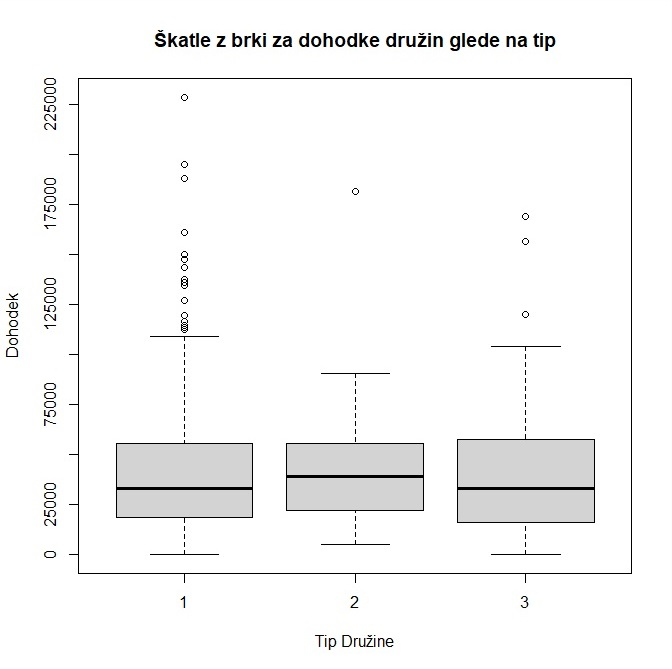
\includegraphics[scale = 0.35]{TabelaSample1}
		\caption{Vzporedno narisane škatle z brki tipov družin $1$, $2$ in $3$}
	\end{figure}
%	\newpage
	Škatle z brki nam ponudijo nekaj zanimivih ugotovitev. V minimalnih dohodkih ni velikih odstopanj, razen pri tipu $2$, ki ima za razliko od ostalih pozitiven minimalen dohodek. Če ignoriramo ostale vzorce in tem rezultatom naivno verjamemo, so enostarševske družine z očetom (torej družine tipa $2$) relativno bolj premožne od ostalih tipov. To domnevo podpira tudi opazka, da je povprečna vrednost tipa $2$ višja kot povprečni vrednosti ostalih dveh tipov, kar lahko preberemo iz izpisa na konzoli. 

	Vrednosti so hkrati tudi dostopne v spodnji tabeli. 

	\begin{table}[h!]
		\label{tab: MeanSDA}
		\centering
		\begin{tabular}{|l|c|c|c|}
			\hline
			Tip & $1$ & $2$ & $3$ \\ \hline
			Povprečje & $41655$ & $46301$ & $39931$ \\ \hline
			SD & $32974{,}23$ & $39500{,}3$ & $31069{,}71$ \\ \hline
		\end{tabular}
	\caption{Povprečne vrednosti in standardni odkloni dohodkov po tipih}
	\end{table}

	Če ne bi imeli že izračunanih povprečij, bi lahko še vedno sklepali o njihovih velikostih s pomoćjo škatel z brki. Opazimo namreč, da se prvi kvartili nahajajo na približno enaki višini z maksimalno razliko v okolici $6000$ v prid družinam tipa $2$, kar velja tudi za mediane. Šele pri tretjem kvartilu ostala dva tipa premagata tip $2$, a tudi tu je največja razlika v rangu $4000$. V tem primeru tipu $2$ pomaga to, da ima izmed vseh tipov družin najmanjšo razdaljo med tretjim kvartilom in mediano, kar pomeni, da so vrednosti, ki pripadajo temu intervalu, bolj gosto porazdeljene.

	Višje povprečje dohodka družin tipa $2$ ni edino, kar izstopa pri škatlah z brki. Družine tipa $1$ izstopajo v tem, da imajo, v primerjavi z ostalimi tipi, veliko število osamelcev (torej tistih vrednosti, ki so na sliki označene s krogi izven škatel).

	Družine tipa $3$ se odlikujejo po tem, da imajo najširši interkvartilni razmik. Za lažji pregled in primerjavo, so vsi interkvartilni razmiki navedeni v konzoli (po pogonu skripte) ter v tabeli spodaj:
	\begin{table}[h!]
		\label{tab: IQRA}
		\centering
		\begin{tabular}{|l|c|c|c|}
			\hline
			Tip & $1$ & $2$ & $3$ \\ \hline
			IQR & $36660$ & $32848$ & $41560$ \\ \hline
		\end{tabular}
		\caption{Interkvartilni razmiki dohodkov po tipih}
	\end{table}

	Družine tipa $2$ so torej v povprečju bolj premožne od družin ostalih tipov in družine tipa $3$ so v povprečju najmanj premožne. Vrednosti družin tipa $3$ so hkrati tudi najbolj razpršene v >>srednji polovici<<, kar nam pove velikost interkvartilnega razmika. Družine tipa $1$ se v obeh primerih nahajajo v sredini med družinami tipa $2$ in $3$. Hkrati imajo tudi razmeroma več osamelcev od ostalih tipov. V vsakem primeru nam rezultati namigujejo, da obstaja povezava med tipom družine in njenim dohodkom.
	\newpage
	\subsection{Primerjava dohodkov družin tipa $1$ v petih vzorcih}\label{subsect: 1B}
	Da nadaljujemo analizo podatkov si oglejmo porazdelitev dohodkov družin nekega tipa preko 5 neodvisno izbranih vzorcev. Pri tem za prvega vzamemo kar vzorec, ki smo ga obravnavali v prejšnjem podpoglavju, ostale štiri pa pridobimo s pomočjo orodij v LibreOffice Calc. Vsi vzorci so posebej shranjeni v lastni datoteki tipa \textit{.csv} z imeni tipa \textit{KibergradVzorec$\#$.csv}.

	Da izrišemo škatle z brki, s pomočjo katerih bomo primerjali dohodke preko vzorcev, poženemo skripto \textit{Kibergrad\_b.R}. V njej najprej naložimo vzorce, nato vsakemu vzorcu dodamo stolpec vrednosti, ki nam pove kateremu vzorcu pripada dan podatek. Torej vzorcu $1$ dodamo stolpec samih enk, vzorcu $2$ stolpec samih dvojk itd. Te tabele nato združimo v eno samo tabelo, iz nje prefiltriramo družine vseh tipov razen $1$ in nato s pomočjo te nove tabele po enakem postopku kot v prejšnjem podpoglavju primerjamo dohodke družin glede na vzorec.

	Dobljene škatle z brki so prikazane spodaj.

	\begin{figure}[h!]
		\label{fig: boxplotB1}
		\centering
		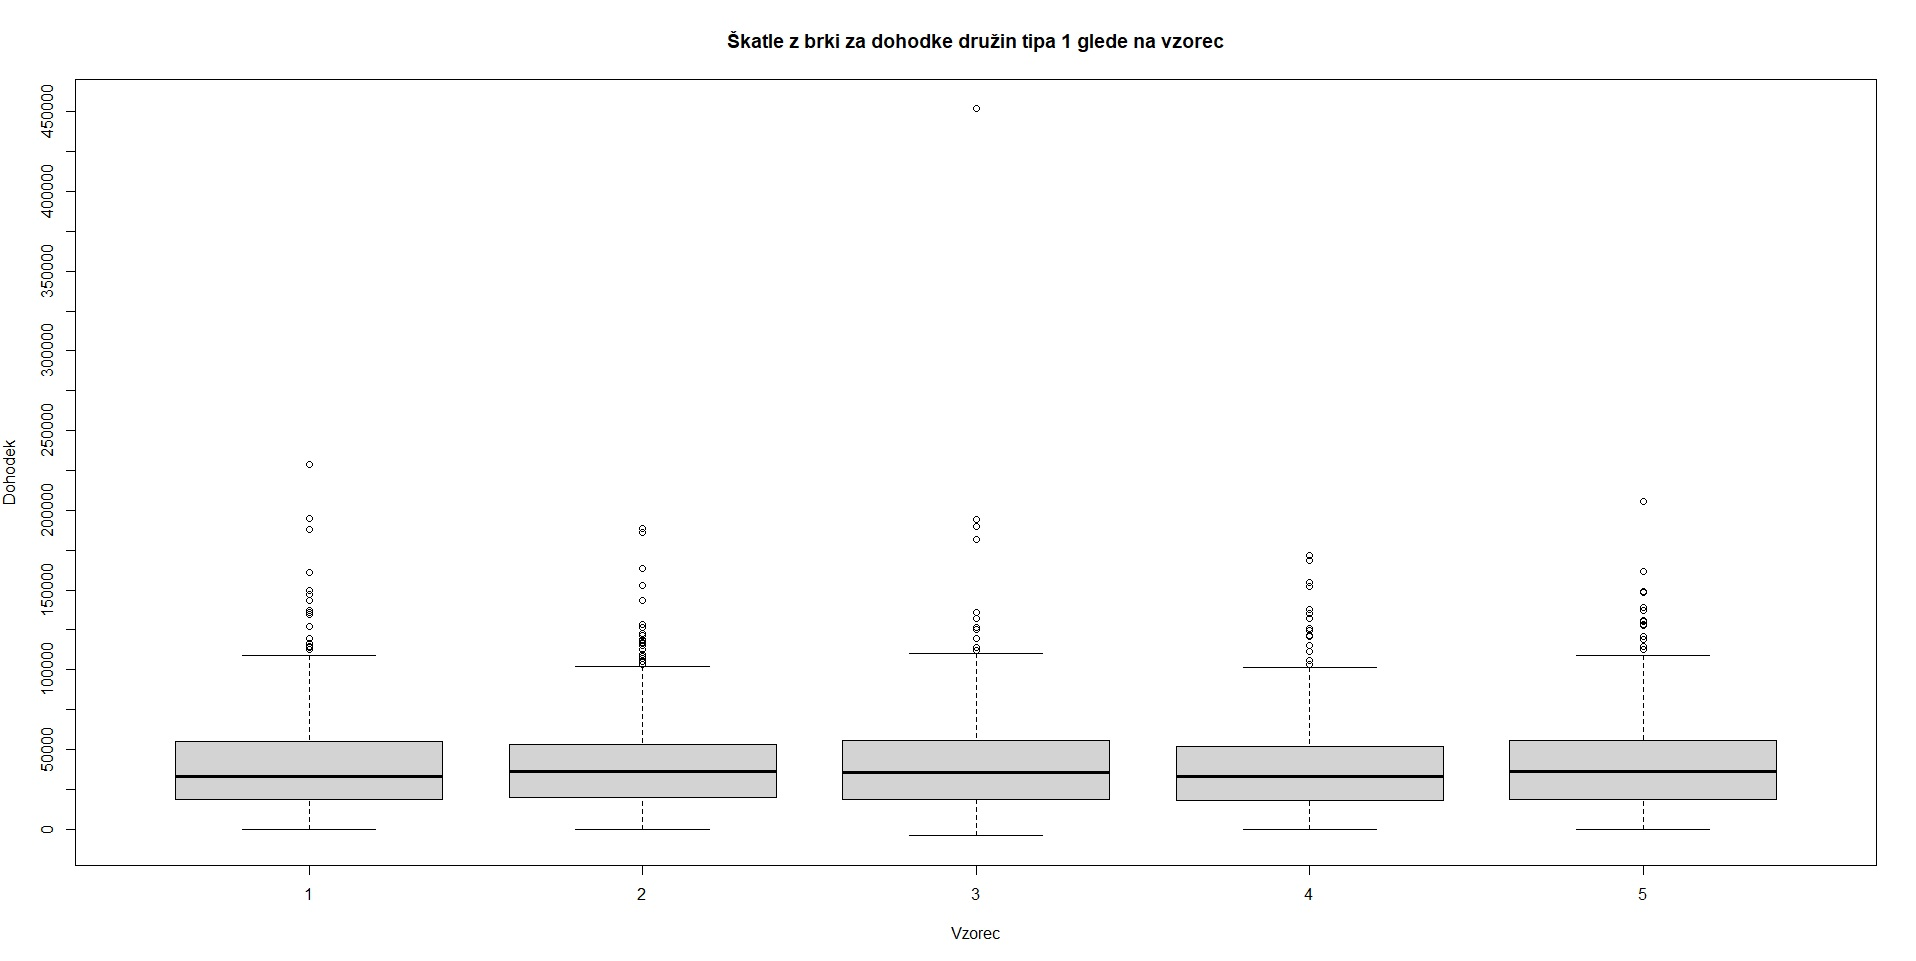
\includegraphics[scale = 0.425]{SkatlezbrkiB}
		\caption{Vzporedno narisane škatle z brki družin tipa $1$ po vzorcih}
	\end{figure}

	Takoj opazimo, da je prikazan graf razpotegnjen, v glavnem na račun enega osamelca iz tretjega vzorca. Da dobimo bolj pregleden graf, odstranimo vse vrednosti, ki so večje od $250000$ (v resnici je taka zgolj ena). Škatle z brki, ki jih dobimo po tem popravku in so prikazane spodaj, skripta samostojno izriše.
	\newpage
	\begin{figure}[h!]
		\label{fig: boxplotB2}
		\centering
		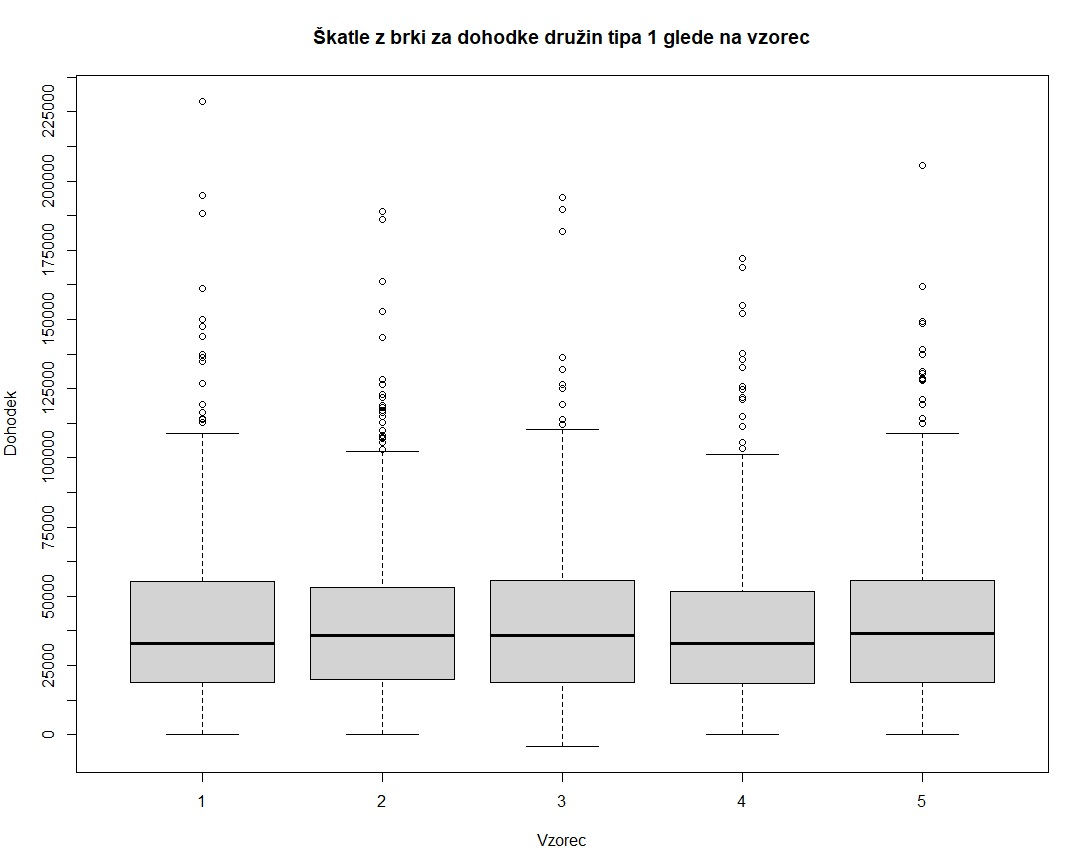
\includegraphics[scale = 0.4]{LepseSkatlezbrkiB}
		\caption{Popravljene vzporedno narisane škatle z brki družin tipa $1$ po vzorcih}
	\end{figure}
	
	Ker smo pri >>popravku<< zanemarili zgolj eno vrednost, nam to bistveno ne pokvari primerjave. Izoliran osamelec bi lahko na našo obravnavo vplival kvečjemu negativno. Zato bomo pri izračunu povprečja za vsak vzorec uporabili tabelo, ki tega osamelca ne vsebuje.
	
	Vrednosti (kvartili, povprečja, maksimalna in minimalna vrednost, IQR), ki jih skripta izpiše v konzolo, so prikazane v spodnji tabeli:
	
	\begin{table}[h!]
		\label{tab: QuartMeanA}
		\centering
		\begin{tabular}{|l|c|c|c|c|c|}
			\hline
			 & Vzorec $1$ & Vzorec $2$ & Vzorec $3$ & Vzorec $4$ & Vzorec $5$ \\ \hline
			Max & $228727$ & $188899$ & $194230$ & $171999$ & $205712$ \\ \hline
			Q$3$ & $55360$ & $53121$ & $55700$ & $51700$ & $55863$ \\ \hline
			Med & $32975$ & $36000$ & $35850$ & $33006$ & $36527$ \\ \hline
			Q$1$ & $18700$ & $20008$ & $18800$ & $18327$ & $18668$ \\ \hline
			Min & $0$ & $0$ & $-4198$ & $0$ & $0$ \\ \hline
			\hline
			Povprečje & $41655$ & $41822$ & $41337$ & $39344$ & $41697$ \\ \hline
			SD & $32974{,}23$ & $31037{,}97$ & $30517{,}25$ & $29867{,}4$ & $31099{,}04$ \\ \hline
			IQR & $36660$ & $33113$ & $36900$ & $33373$ & $37195$ \\ \hline
		\end{tabular}
		\caption{Ekstremi, kvartili, povprečja, standardni odkloni in interkvartilni razmiki dohodkov družin tipa $1$ po vzorcih}
	\end{table}
	
	Sedaj, ko imamo narisane škatle z brki in zraven napisano tabelo, lahko komentiramo rezultate. V prvi vrsti opazimo, da so si povprečja dokaj blizu. Vsa povprečja razen povprečje četrtega vzorca se nahajajo v okolici $41500 \pm 500$, povprečje vzorca $4$ pa se od $41500$ razlikuje za manj kot $2500$. Če bi si izbrali še već vzorcev, bi se po vsej verjetnosti njihova povprečja tudi nahajala v neki bližnji okolici $41500$. Podobno obnašanje standardnih odklonov, ki se nabirajo v okolici $31000 \pm 2000$ nas privede do nepresenetljivega sklepa, da je porazdelitev dohodka družin tipa $1$ neodvisna od vzorca. To potrjuje tudi relativna bližina kvartilov v tabeli (npr. tretji kvartili se zbirajo v okolici $53000 \pm 3000$).
	
	Na tej točki bi želeli preveriti, ali je porazdelitev slučajno normalna. Test s primerjalnim kvartilnim grafikonom na vzorcu $1$ nam pove, da to ne drži. Enak sklep seveda velja tudi za ostale vzorce. Zakomentiran ukaz za izris spodnjega grafikona se nahaja na koncu skripte \textit{Kibergrad\_b.R}. Ukaz je zakomentiran zato, da program raje izriše grafikon škatel z brki, na katerih je povdarek te naloge.
	
	\begin{figure}[h!]
		\label{fig: qqplotB}
		\centering
		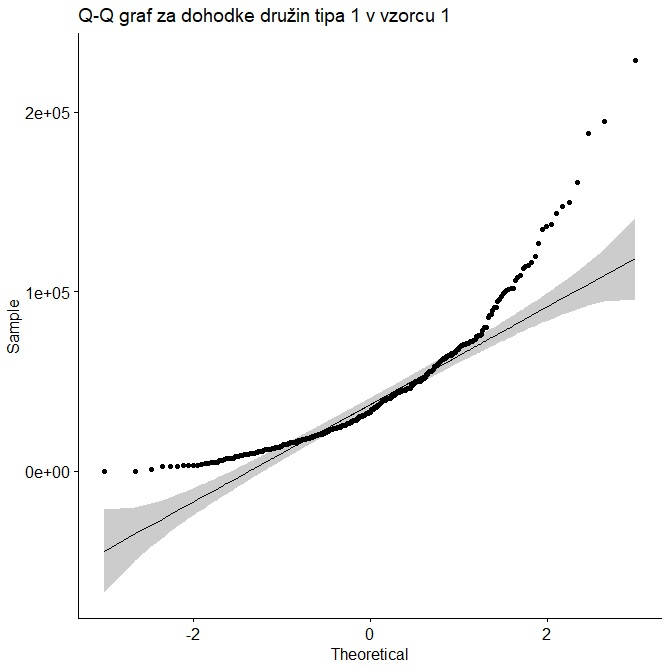
\includegraphics[scale = 0.5]{QQVzorec1}
		\caption{Primerjalni kvartilni grafikon dohodkov družin tipa $1$ v vzorcu 1}
	\end{figure}
	
	Četudi dohodki niso porazdeljeni normalno, so še vedno razmeroma konsistentni preko obravnavanih vzorcev. To je v kontrastu z razlikami in odstopanji, ki smo jih opazili, ko smo v prvem vzorcu primerjali dohodke glede na tip družine. Ta kontrast dodatno potrjuje sklep, da tip družine netrivialno vpliva na dohodek družine. 
	
	\subsection{S tipom pojasnjena varianca populacije}\label{subsect: 1C}
	Na koncu prejšnjega podpoglavja smo prišli do sklepa, da ima tip družine netrivialen vpliv na dohodek družine. Če to drži ali ne, lahko preverimo z izračunom s tipom družine pojesnjene variance. Čim smo poračunali to, se lahko skličemo na zvezo med varianco in pojasnjeno ter nepojasnjeno varianco ($Celotna\_varianca = Pojasnjena\_varianca + Nepojasnjena\_varianca$) in poračunamo še slednjo. Vsi računi in primerjave se prikažejo ob pogonu skripte \textit{Kibergrad\_c.R}. 
	
	Z $n_i$ označimo število družin tipa $i$ ter z $N$ velikost naše populacije. Z $X$ označimo dohodke družin, z $Y$ pa  slučajno spremenljivko tipov družin, ki ima porazdelitev $P(Y = i) = n_i / N$. Predpostavimo, da so dohodki tipov družin $X_i = X_{|Y=i}$ medseboj neodvisni. Predpostavko upravičimo z argumentom, da v splošnem dohodek soseda ne vpliva na naš dohodek. Pomnimo tudi, da je $E\left[X|Y\right]$ neka funkcija spremenljivke $Y$, recimo $\Phi(Y)$.
	Z $\bar{X}_i$ še označimo pričakovano vrednost dohodka v družini tipa $i$, torej $\bar{X}_i = E\left[X|Y = i\right]$. S tipom pojasnjeno varianco potem izračunamo po formuli: 
	\begin{equation*} \label{eq: explvarC} \begin{split}
			& Var(E\left[X|Y\right]) = Var(\Phi(Y)) = E\left[(\Phi(Y)- E\left[\Phi(Y)\right])^2\right] =\\ 
			&= \sum_{i = 1}^{3} (\Phi(Y = i)- E\left[\Phi(Y)\right])^2 * P(Y = i) = \\ &= 1/N * \sum_{i = 1}^{3} n_i * (E\left[X|Y = i\right] - E\left[E\left[X|Y\right]\right])^2 = \\ &= 1/N * \sum_{i = 1}^{3} n_i * (\bar{X}_i - E\left[X\right])^2 = 1/N * \sum_{i = 1}^{3} n_i * (\bar{X}_i - \bar{X})^2
		\end{split}
	\end{equation*}

	S pomočjo zgoraj pridobljene formule v \textit{Kibergrad\_c.R} poračunamo pojasnjeno varianco. Nepojasnjeno varianco nato poračunamo kot razliko populacijske variance in pojasnjene variance. Vrednosti skripta izpiše v konzolo, dostopne pa so tudi v spodnji tabeli.
	
	\begin{table}[h!]
		\label{tab: varC}
		\centering
		\begin{tabular}{|l|c|}
			\hline
			Varianca & $1026385670$ \\ \hline
			Pojasnjena & $113781162$ \\ \hline
			Nepojasnjena & $912604508$ \\ \hline
			SD & $32037{,}2544062437$ \\ \hline
		\end{tabular}
		\caption{Populacijska, s tipi pojasnjena in nepojasnjena varianca}
	\end{table}
	
	Opazimo, da je nepojasnjena varianca bistveno višja od pojasnjene variance. Če pogledamo delež, ki ga varianci zavzemata, nam s tipi družin pojasnjena varianca predstavlja le približno $11{,}09\%$. To nam pove, da je tip družine netrivialen faktor pri napovedi dohodka družine, ni pa glavni faktor. To se ujema s tem, kar smo razbrali v prejšnjih podpoglavjih. Že zgolj za družine tipa $1$ v podpoglavju \ref{subsect: 1B} je bil standardni odklon, torej koren variance, razmeroma visok v vsakem vzorcu. To se ujema s tem, da večino variance pridobimo od faktorjev, ki niso tip družine. Če bi tip družine bil odgovoren za večji delež celotne variance dohodkov, bi bila varianca znotaj tipov manjša.
	
	\section{Slučajni sprehod} \label{sect: SlucajniSprehod}
	Za začetek omenimo, da se podatki, ki so uporabljeni v tem delu naloge, vsebovani v datotekah \textit{Kromatin\_kratki.csv}, \textit{Kromatin\_srednji.csv} in \textit{Kromatin\_dolgi.csv}. Ti podatki so razdalje med pari zaporedij nukleotidov, ki so bile izmerjene v treh različnih eksperimentih. Spomnimo se tudi, da imajo te razdalje Rayleighovo porazdelitev, ki je podana z gostoto \begin{equation*}\label{eq: RayleighDist}
		f(r|\theta) = \begin{cases}
			\frac{r}{\theta^2}\exp\big(-\frac{r^2}{2\theta^2}\big)~;~r>0 \\
			0~;~\text{sicer}
		\end{cases}
	\end{equation*}
	V prvih dveh podpoglavjih, torej \ref{subsect: 2A} in \ref{subsect: 2B}, določili cenilki za $\theta$ po metodi največjega verjetja in po metodi momentov. Nato bomo za obe pridobljeni cenilki ugotovili, ali sta nepristranski oz. katera je vsaj asimptotično bolj nepristranska. Pri tem bomo uporabili izračun asimptotične srednje kvadratične napake oz. $MSE$. V preostalih delih bomo konkretno uporabili priložene datoteke z meritvami, najprej da določimo numerične ocene cenilk za vsak eksperiment (torej vsako datoteko) posebej. Za vse izračune bomo tudi ocenili standardno napako in rezultate grafično prikazali. Na koncu bomo pridobljeni gostoti primerjali s histogramom meritev.
	\subsection{Cenilka za $\theta$ po metodi največjega verjetja} \label{subsect: 2A}
	Denimo, da imamo $n$ medseboj neodvisnih in enako porazdeljenih spremenljivk $X_i~;~i\in\{1, 2, \ldots, n\}$, ki so vse porazdeljene z Rayleighovo porazdelitvijo \ref{eq: RayleighDist}. Verjetje definiramo s predpisom \begin{equation*}
		L(\theta | x_1, \ldots, x_n) = \prod_{i = 1}^{n} f_{X_i}(x_i | \theta) = \begin{cases}
			\prod_{i = 1}^{n} \frac{x_i}{\theta^2}\exp\big(-\frac{x_i^2}{2\theta^2}\big)~;~ x_1, \ldots, x_n > 0 \\
			0~;~\text{sicer}
		\end{cases}
	\end{equation*}
	Ker je lahko delo s tem produktom zahtevno, raje vse skupaj logaritmiramo in dobimo $$l(\theta|x_1,\ldots, x_n) = \sum_{i = 1}^{n} \ln(\frac{x_i}{\theta^2}) - \frac{x_i^2}{2\theta^2}~;~\textit{za}~ x_1,\ldots,x_n >0$$
	
	Cenilka $\theta$ po metodi največjega verjetja je neka funkcija $h(X_1,\ldots, X_n)$ pri kateri $L(\theta|x_1,\ldots, x_n)$ doseže maksimum za vse $X_1,\ldots, X_n$. Logaritmiranje $L$ ohrani ta ekstrem v smislu, da če bo $L$ dosegel svoj maksimum v $\theta$, bo tam svoj maksimum dosegel tudi $l$ in obratno.
	Sedaj odvajamo $l$ po $\theta$ in dobimo: \begin{equation*}\label{eq: Verjetje}
		\frac{\partial l}{\partial\theta} (\theta | x_1,\ldots, x_n) = \sum_{i = 1}^{n} \big(\frac{-2 * \theta^2 * x_i}{\theta^3 * x_i} - \frac{-2 * x_i^2}{2 * \theta^3}\big) = \sum_{i = 1}^{n} \big(\frac{x_i^2}{\theta^3} - \frac{2}{\theta} \big)= \sum_{i = 1}^{n} \big(\frac{x_i^2}{\theta^3}\big) - \frac{2 * n}{\theta}
	\end{equation*}
	Da najdemo ekstrem moramo rešiti enačbo $\frac{\partial l}{\partial\theta} (\theta | x_1,\ldots, x_n) = 0$. Ko vanjo vstavimo, kar smo ravnokar poračunali zgoraj, dobimo $$
		\sum_{i = 1}^{n}\frac{x_i^2}{\theta^3} = \frac{2*n}{\theta}
	$$
	oziroma $$\sum_{i = 1}^{n}x_i^2 = 2*n*\theta^2$$ Od tod izrazimo $\theta^2$ iz zgornje enakosti in rezultat korenimo, da dobimo $\theta$. Velja: $$\theta = \pm \sqrt{\frac{\sum_{i = 1}^{n}x_i^2}{2 * n}}$$ Preveriti moramo še, da $l$ v $\theta$ res doseže maksimum. Za to poračunamo drugi odvod $l$ po $\theta$: $$\frac{\partial^2 l}{\partial\theta^2}(\theta | x_1, \ldots, x_n) = \sum_{i = 1}^{n} (-3)\frac{x_i^2}{\theta^4} + \frac{2n}{\theta^2}$$ 
	Sedaj v izraz vstavimo $\theta = \pm \sqrt{\frac{\sum_{i = 1}^{n}x_i^2}{2 * n}}$ in tako dobimo $$\sum_{i=1}^{n} (-3)\frac{4 n^2 x_i^2}{(\sum_{i = 1}^{n}x_i^2)^2} + \frac{4n^2}{\sum_{i=1}^{n}x_i^2} = \frac{4n^2}{\sum_{i=1}^{n}x_i^2}(\frac{(-3)\sum_{i=1}^{n}x_i^2}{\sum_{i = 1}^{n}x_i^2} +1) = (-2)\frac{4n^2}{\sum_{i=1}^{n}x_i^2} < 0$$
	
	Ugotovili smo že, da ima verjetje $l$ ekstrema v $+\sqrt{\frac{\sum_{i = 1}^{n}x_i^2}{2n}}$ in $-\sqrt{\frac{\sum_{i = 1}^{n}x_i^2}{2n}}$, sedaj pa vemo tudi, da sta oba ekstrema maksimuma. Za cenilko $\theta$ po metodi največjega verjetja izberemo koren s pozitivnim predznakom. Cenilka $\theta$ po metodi največjega verjetja je torej $\widehat{\theta} = \sqrt{\frac{\sum_{i = 1}^{n}X_i^2}{2 * n}}$. Vrednost cenilke je odvisna od števila spremenljivk. Bolj primerna je torej oznaka $\widehat{\theta}_n = \sqrt{\frac{\sum_{i = 1}^{n}X_i^2}{2 * n}}$.
	
	\subsection{Cenilka za $\theta$ po metodi momentov}\label{subsect: 2B}
	Sedaj se obrnemo na metodo momentov. Denimo, da so $X_1,\ldots, X_n$ neodvisne enako porazdeljene slučajne spremenljivke. Da določimo cenilko za izbrane parametre po tej metodi, moramo najprej poračunati momente nizkih stopenj, torej $E\left[X^k\right]$, v odvisnosti od parametrov, ki jih želimo oceniti. Nato iz dobljenih enačb izrazimo parametre v odvisnosti od momentov. Cenilko za parametre dobimo tako, da v enačbi $k$-ti moment zamenjamo s povprečjem $k$-tih potenc $\frac{1}{n}\sum_{i=1}^{n}X_i^k$. Ker v našem primeru skušamo oceniti samo en paramater, $\theta$, načeloma zadošča če izračunamo samo prvi moment.
	
	\begin{equation*}
		E\left[X\right] = \int_{-\infty}^{\infty}x f(x|\theta)\,dx = \int_{0}^{\infty} \frac{x^2}{\theta^2}e^{-\frac{x^2}{2\theta^2}}\,dx
	\end{equation*}
	Uvedemo novo spremenljivko $u =\frac{x^2}{2\theta^2}~;~du = \frac{x}{\theta^2}\,dx$, torej je~$dx = \frac{\theta^2}{x} du$. Naš integral nato postane:
	\begin{equation*}
		\int_{0}^{\infty} x e^{-u}\,du = \int_{0}^{\infty} \sqrt{2u\theta^2} e^{-u}\,du = \theta\sqrt{2} \int_{0}^{\infty} u^{\frac{1}{2}}e^{-u}\,du
	\end{equation*}
	V integralu prepoznamo obliko gama funkcije in hitro ugotovimo, da je integral enak $\Gamma(\frac{3}{2}) = \frac{1}{2}\sqrt{\pi}$.
	
	Sledi, da je pričakovana vrednost Rayleighove porazdelitve s parametrom $\theta$ enaka $\sqrt{\frac{\pi}{2}}\theta$. Od tod izrazimo $\theta$ kot $\theta = \sqrt{\frac{2}{\pi}}E\left[X\right]$. Cenilka $\theta$ po metodi momentov je torej $\widehat{\theta} = \sqrt{\frac{2}{\pi}}\bar{X} = \frac{\sqrt{2}}{n\sqrt{\pi}}\sum_{i=1}^{n}X_i$.
	Tudi v tem primeru nam število spremenljivk vpliva na vrednost cenilke. Zato smo v resnici pridobili celo zaporedje cenilk $\widehat{\theta}_n$, tako kot v prejšnjem podpoglavju.

	\subsection{Asimptotični $MSE$ cenilk}\label{subsect: 2C}
	Srednja kvadratična napaka cenilke definirana s formulo $MSE(\widehat{\theta}|\theta) = E[(\widehat{\theta} - \theta)^2]$. Da izračunamo asimptotično $MSE$, najprej za fiksen $n$ poračunamo $MSE$, nato pa dobljeno limitiramo: $\lim_{n\mapsto\infty}MSE(\widehat{\theta}_n | \theta)$. Pri računanju nam tudi pomaga enakost $MSE(\widehat{\theta} | \theta) = Var(\widehat{\theta}) + Bias(\widehat{\theta}|\theta)^2$.
	Pri tem se pristranskost oz >>Bias<< izračuna po formuli $Bias(\widehat{\theta}|\theta) = E[\widehat{\theta}] - \theta$.
	\subsubsection{MSE cenilke po metodi največjega verjetja}\label{subsubsect: 2C1}
	Začnimo s cenilko, ki smo jo pridobili po metodi največjega verjetja. Najprej za fiksen $n$ poračunamo pristranskost. Pri tem nam pomaga informacija, ki smo jo pridobili iz vira \cite{bib:Rayleigh}, da ima $Y = \sum_{i = 1}^{n} X_i^2$ gama porazdelitev $\Gamma(n, \frac{1}{2*\theta^2})$.
	\begin{equation*}
		E[\widehat{\theta}_n] = E[\frac{1}{\sqrt{2n}}\sqrt{Y}] = \frac{1}{\sqrt{2n}} E[\sqrt{Y}]
	\end{equation*}
	Poračunajmo sedaj $E[\sqrt{Y}]$.
	\begin{equation*}
		E[\sqrt{Y}] =  \int_{0}^{\infty}\sqrt{y}\frac{(\frac{1}{2\theta^2})^n}{\Gamma(n)}y^{n-1}e^{-\frac{y}{2\theta^2}}\, dy = \int_{0}^{\infty}(\frac{y}{2\theta^{2}})^n\frac{1}{\Gamma(n)\sqrt{y}} e^{-\frac{y}{2\theta^2}}\,dy
	\end{equation*}
	Vstavimo novo spremenljivko $u = \frac{y}{2\theta^2}~;~du = \frac{1}{2\theta^2}\, dy$. Pri tem še opazimo, da je $\sqrt{y} = \sqrt{2\theta^2 u}$. Sedaj vstavimo to v integral.
	
	\begin{equation*}
		E[\sqrt{Y}] = \int_{0}^{\infty} u^n \frac{1}{\Gamma(n)\sqrt{2\theta^2}\sqrt{u}} e^{-u} 2\theta^2\,du = \frac{\sqrt{2\theta^2}}{\Gamma(n)} \int_{0}^{\infty} u^{n - \frac{1}{2}} e^{-u}\,du = \sqrt{2\theta^2}\frac{\Gamma(n+\frac{1}{2})}{\Gamma(n)}
	\end{equation*}
	Sledi, da je $E[\widehat{\theta}_n] = \frac{\theta\Gamma(n + \frac{1}{2})}{\sqrt{n}\Gamma(n)}$ in potem je $\widehat{\theta}_n$ pristranska cenilka, saj je $$E[\widehat{\theta}_n] - \theta = \theta (\frac{\Gamma(n + \frac{1}{2})}{\sqrt{n}\Gamma(n)} - 1) \neq 0$$ za $\theta\neq 0$. Cenilko lahko popravimo na nepristransko. Nepristranska cenilka je tako $$\theta_n^+ = \frac{\Gamma(n)\sqrt{n}}{\Gamma(n + \frac{1}{2})}\widehat{\theta}_n = \frac{\Gamma(n)}{\Gamma(n + \frac{1}{2})\sqrt{2}}\sqrt{Y}$$
	Uspelo nam je torej izračunati pristranskost naše cenilke $\widehat{\theta}_n$: $$Bias(\widehat{\theta}_n) = \theta(\frac{\Gamma(n + \frac{1}{2})}{\sqrt{n}\Gamma(n)} - 1)$$
	
	Ko poračunamo limito $\lim_{n\mapsto\infty} \frac{\Gamma(n + \frac{1}{2})}{\sqrt{n}\Gamma(n)} = 1$, vidimo, da je $\widehat{\theta}_n$ asimptotsko nepristranska, saj sledi $\lim_{n\mapsto\infty}Bias(\widehat{\theta}_n) = 0$. Poračunati moramo še varianco cenilke $Var(\widehat{\theta}_n) = E[\widehat{\theta}_n^2] - E[\widehat{\theta}_n]^2 = E[\frac{1}{2n} Y] - E[\widehat{\theta}_n]^2$. Za Porazdelitev $Y$ vemo, da je $\Gamma(n, \frac{1}{2\theta^2})$, tako da hitro pridobimo $E[\frac{1}{2n} Y] = \frac{1}{2n}\frac{n}{\frac{1}{2\theta^2}} = \frac{1}{2n}2n\theta^2 = \theta^2$. Sledi $$Var(\widehat{\theta}_n) = \theta^2(1 - \frac{\Gamma(n + \frac{1}{2})^2}{n\Gamma(n)^2})$$
	Ko to varianco limitiramo z $n\mapsto\infty$, gre izraz v oklepaju proti $0$, torej je $\lim_{n\mapsto\infty}Var(\widehat{\theta}_n) = 0$. Posledično je asimptotična $MSE(\widehat{\theta}_n)$ enaka $0$, torej $\lim_{n\mapsto\infty}MSE(\widehat{\theta}_n) = 0$.
	
	\subsubsection{MSE cenilke po metodi momentov}\label{subsubsect: 2C2}
	Sedaj storimo enako še za cenilko, ki smo jo pridobili po metodi momentov $\widehat{\theta}_n = \sqrt{\frac{2}{\pi}}\bar{X}$. Najprej poračunajmo njeno pričakovano vrednost.
	
	\begin{equation*}		
		E[\widehat{\theta}_n] = \frac{\sqrt{2}}{n\sqrt{\pi}} \sum_{i=1}^{n} E[X_i] = \sqrt{\frac{2}{\pi}} E[X] = \theta
	\end{equation*}
	
	Od tod lahko že sklepamo, da je $\widehat{\theta}_n$ nepristranska cenilka. Sledi, da je $MSE(\widehat{\theta}_n) = Var(\widehat{\theta}_n)$. Poračunajmo sedaj še varianco in pri tem upoštevamo, da so $X_i$ medseboj neodvisne in enako porazdeljene.
	
	\begin{equation*}		
		Var(\widehat{\theta}_n) = \frac{2}{n^2\pi}Var(\sum_{i = 1}^{n}X_i) = \frac{2}{n^2 \pi} \sum_{i = 1}^{n}Var(x_i) = \frac{2}{n \pi} Var(X)
	\end{equation*}
	
	Na tej točki se skličemo na varianco rayleighove porazdelitve s parametrom $\theta^2$, ki je enaka $\frac{4 - \pi}{2}\theta^2$. Sledi, da je $Var(\widehat{\theta}_n) = \frac{2}{n\pi} * \frac{4 - \pi}{2}\theta^2 = \frac{(4-\pi)}{n\pi}\theta^2$, ki konvergira proti $0$ ko pošljemo $n\mapsto\infty$. Posledično je $\lim_{n\mapsto\infty}MSE(\widehat{\theta}_n) = \lim_{n\mapsto\infty} Var(\widehat{\theta}_n) =0$.
	
	Tako prva kot druga cenilka imata torej asimptotično srednjo kvadratično napako $0$. Kljub temu sklepamo, da je cenilka, ki smo jo pridobili po metodi momentov, boljša od cenilke, ki smo jo pridobili po metodi največjega verjetja, saj je cenilka po metodi momentov zraven še nepristranska.
	
	\subsection{Ševilska ocena prve cenilke} \label{subsect: 2D}
	
	Številsko oceno cenilke za vsak eksperiment izvedemo s pomočjo skripte \textit{SlucajniSprehodiMNV.R}. Ta ob zagonu poračuna številske vrednosti cenilke, oceni standardno napako vsake cenilke ter izriše pripadajoče grafe gostot za vsak eksperiment in graf na katerem so prikazani vsi trije grafi. Pri tem standardno napako $SE(\widehat{\theta}_n)$ cenilke pridobljene po metodi največjega verjetja izračunamo kot $\sqrt{Var(\widehat{\theta}_n)}$. Velja torej, da je $SE(\widehat{\theta}_n) = \theta\sqrt{1 - \frac{\Gamma(n + \frac{1}{2})^2}{n\Gamma(n)^2}}$. Ker parametra $\theta$ ne poznamo, izračunamo cenilko za $SE$ po formuli $\widehat{SE}(\widehat{\theta}_n) = \widehat{\theta}_n \sqrt{1 - \frac{\Gamma(n + \frac{1}{2})^2}{n\Gamma(n)^2}}$
	Prej omenjena skripta ocenjene vrednosti cenilk in standardnih napak izpiše v konzolo, so pa zbrane tudi v spodnji tabeli, ki pa vsebuje tudi na dve decimalki zaokrožene vrednosti standardnih napak.
	
	\begin{table}[h!]
		\label{tab: mnvse}
		\centering
		\begin{tabular}{|l|c|c|c|}
			\hline
			Eksperiment & kratki & srednji & dolgi \\ \hline
			Vrednost $\widehat{\theta}$ & $1{,}117394$ & $2{,}075983$ & $3{,}324422$ \\ \hline
			Ocena SE & $0{,}05728327$ & $0{,}0658959$ & $0{,}1451586$ \\ \hline
		\end{tabular}
		\caption{Numerične vrednosti MNV cenilke in standardne napake po eksperimentih}
	\end{table}
	
	Izračun standardne napake cenilke je neizogiben in pomemben del vsake statistične analize podatkov. Razlog za to je, ker nam služi kot merilo, kako dobro se naša cenilka prilega dejanskemu parametru, ki ga cenimo glede na dane podatke. Če je standardna napaka velika, vrednosti cenilke močno odstopajo od pričakovane vrednosti cenilke, ki je, v primeru ko je cenilka nepristranska, ravno enaka populacijskemu parametru, ki ga ocenjuje. Iz tega razloga, se načeloma raje dela z nepristranskimi cenilkami. Vseeno enaka intuicija velja tudi za pristranske spremenljivke - večja kot je standardna napaka na vzorcu, bolj odstopa cenilka od dejanske vrednosti parametra, ki ga ocenjujemo, za celotno populacijo in manjša kot je standardna napaka, manj cenilka odstopa od dejanske vrednosti parametra.
	
	Kot je bilo že prej omenjeno, skripta \textit{SlucajniSprehodiMNV.R} tudi nariše grafe verjetij, ki pripadajo izračunanim ocenam paramatra $\theta$. Na teh grafih je z zeleno črto označena izračunana vrednost $\theta$, okoli nje pa je z rdečima črtkanima premicama označena pripadajoča $SE$-okolica. Skripta sicer grafe izriše enega zraven drugega, tukaj pa bodo priloženi vsak posebej.
	
	\begin{figure}[h!]
		\label{fig: 2Dplot1}
		\centering
		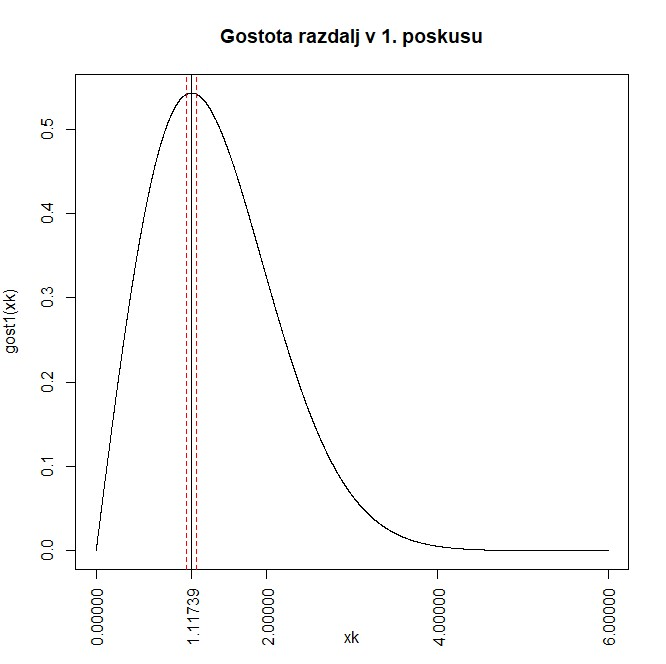
\includegraphics[scale = 0.375]{VerjetjeMNV1}
		\caption{Verjetje za oceno cenilke $\theta$, pridobljene po metodi največjega verjetja, v prvem poskusu}
	\end{figure}

	\begin{figure}[h!]
		\label{fig: 2Dplot2}
		\centering
		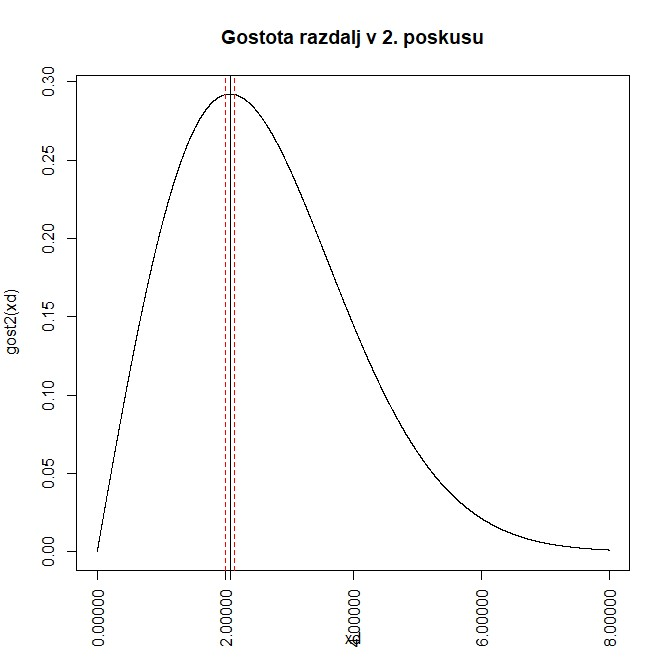
\includegraphics[scale = 0.375]{VerjetjeMNV2}
		\caption{Verjetje za oceno cenilke $\theta$, pridobljene po metodi največjega verjetja, v drugem poskusu}
	\end{figure}

	\begin{figure}[h!]
		\label{fig: 2Dplot3}
		\centering
		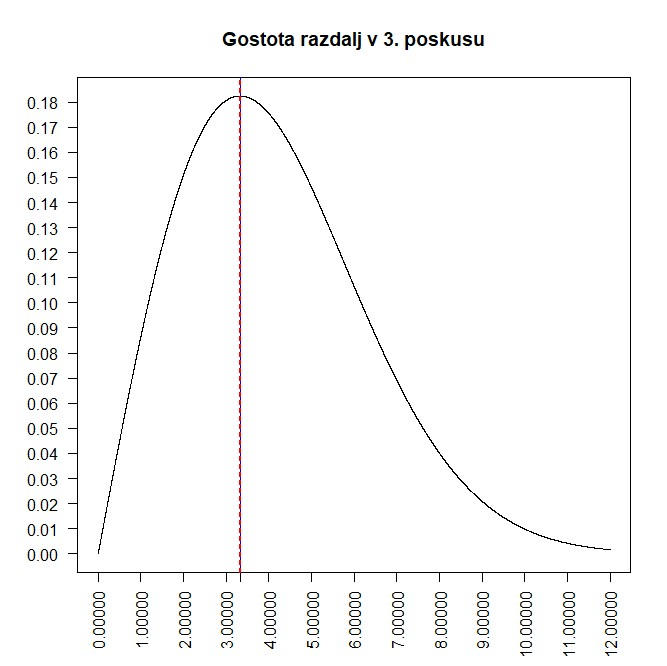
\includegraphics[scale = 0.375]{VerjetjeMNV3}
		\caption{Verjetje za oceno cenilke $\theta$, pridobljene po metodi največjega verjetja, v tretjem poskusu}
	\end{figure}

	Skripta dodatno vrne graf, na katerem so narisane vse tri zgoraj prikazane gostote, skupaj z oznakami njihovih pripadajočih vrednosti cenilk $\widehat{\theta}$ in pripadajočimi $SE$-okolicami. Namen tega zadnjega grafa je prikazati, kako izgledajo gostote, ko jih postavimo v isti koordinatni sistem in na podlagi tega omogočiti primerjavo.
	
	\begin{figure}[h!]
		\label{fig: 2Dplot4}
		\centering
		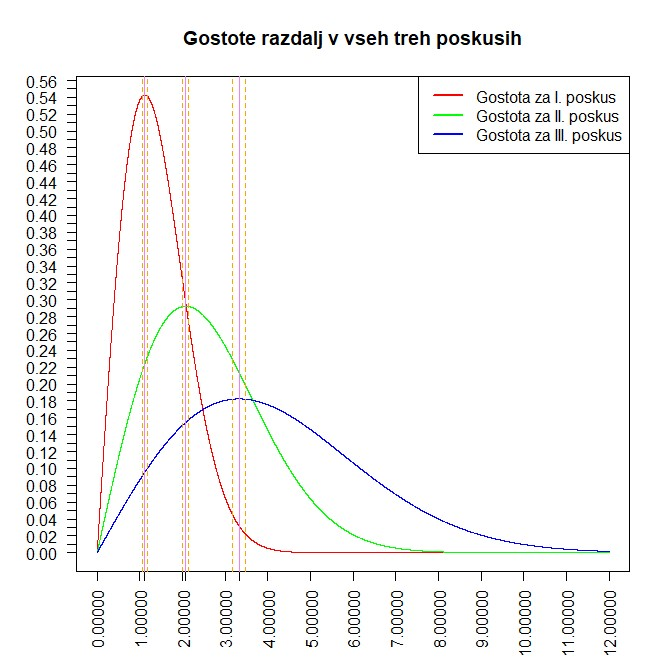
\includegraphics[scale = 0.35]{VerjetjeMNV4}
		\caption{Verjetja za vse ocene cenilke $\theta$, pridobljene po metodi največjega verjetja}
	\end{figure}
	
	Na vsakem grafu verjetja vidimo, da je $SE$-okolica pripadajoče izračunane cenilke razmeroma majhna in vsebuje maksimum verjetja, kar nas ne preseneti, saj je to smiselno za cenilko pridobljeno po metodi največjega verjetja. Dodatno opazimo, da verjetja postajajo bolj položna z zaporednimi poskusi. Razlog za to je naraščanje velikosti posameznih meritev v zaporednih poskusih kar poveča numerično vrednost cenilke. Obnašanje grafov gostot je torej popolnoma normalno, saj velja, da večji kot je parameter $\theta$, bolj položen bo graf gostote Rayleighove porazdelitve za ta parameter. 
	Zaradi razmeroma majhne velikosti standardnih napak lahko sklepamo, da je cenilka $\widehat{\theta}$ pridobljena po metodi največjega verjetna dobra cenilka za parameter $\theta$. Seveda jo lahko še izboljšamo, tako da jo popravimo v nepristransko cenilko $\widehat{\theta}^{+}$, ki smo jo izračunali v podpodpoglavju \ref{subsubsect: 2C1}.
	
	\subsection{Številska ocena druge cenilke} \label{subsect: 2E}
	
	Tako kot v poglavju \ref{subsect: 2D}, lahko tudi za cenilko pridobljeno po metodi momentov stnandardno napako poračunamo kar kot koren variance: $SE(\widehat{\theta}_n) = \sqrt{Var(\widehat{\theta}_n)} = \sqrt{\frac{(4-\pi)}{n\pi}\theta^2} = \sqrt{\frac{(4-\pi)}{n\pi}}\theta$. Ker $\theta$ seveda ne poznamo, v izraz vstavimo cenilko $\widehat{\theta}_n$. Tako je naša formula na koncu $SE(\widehat{\theta}_n) = \sqrt{\frac{(4-\pi)}{n\pi}}\widehat{\theta}_n$. Skripta \textit{SlucajniSprehodiMM.R} poračuna oceno cenilke, ki smo jo pridobili po metodi momentov ter standardno napako s pomočjo prej navedene formule. Vrednosti so navedene v spodnji tabeli skupaj z na dve decimalki zaokroženimi vrednostmi standardnih napak.
	
	\begin{table}[h!]
		\label{tab: mmse}
		\centering
		\begin{tabular}{|l|c|c|c|}
			\hline
			Eksperiment & kratki & srednji & dolgi \\ \hline
			Vrednost $\theta$ & $1{,}163652$ & $2{,}068998$ & $3{,}412388$ \\ \hline
			Ocena SE & $0{,}06240695$ & $0{,}06867617$ & $0{,}1558456$ \\ \hline
		\end{tabular}
		\caption{Numerične vrednosti cenilke pridobljene po metodi momentov in standardne napake po eksperimentih}
	\end{table}

	Poleg tega skripta tudi izriše graf gostote za ocenjeno cenilko za vsak poskus. Te grafe izriše enega zraven drugega, spodaj pa so grafi prikazani posebej.
	
	\begin{figure}[h!]
		\label{fig: 2Eplot1}
		\centering
		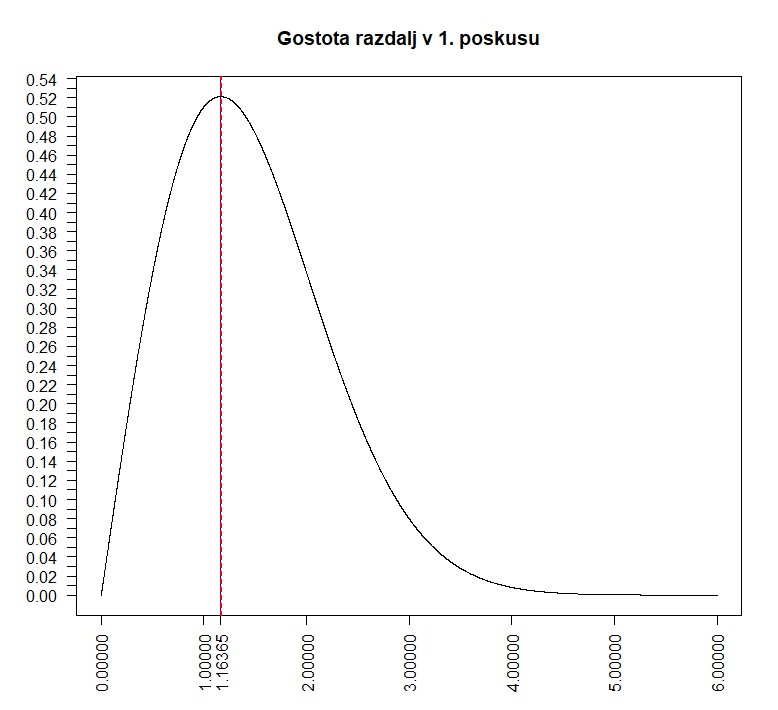
\includegraphics[scale = 0.45]{VerjetjeMM1}
		\caption{Verjetje za oceno cenilke $\theta$, pridobljene po metodi momentov, v prvem poskusu}
	\end{figure}
	
	\begin{figure}[h!]
		\label{fig: 2Eplot2}
		\centering
		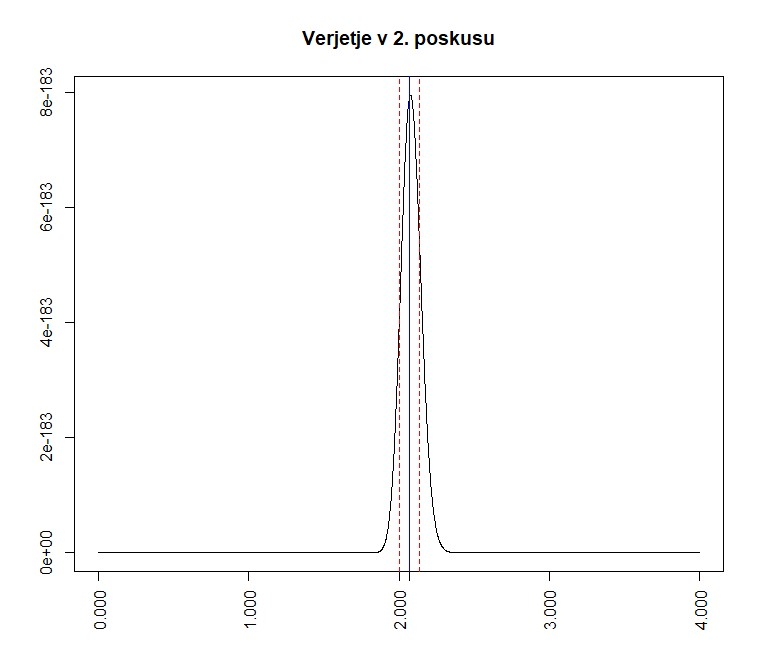
\includegraphics[scale = 0.4]{VerjetjeMM2}
		\caption{Verjetje za oceno cenilke $\theta$, pridobljene po metodi momentov, v drugem poskusu}
	\end{figure}
	
	\begin{figure}[h!]
		\label{fig: 2Eplot3}
		\centering
		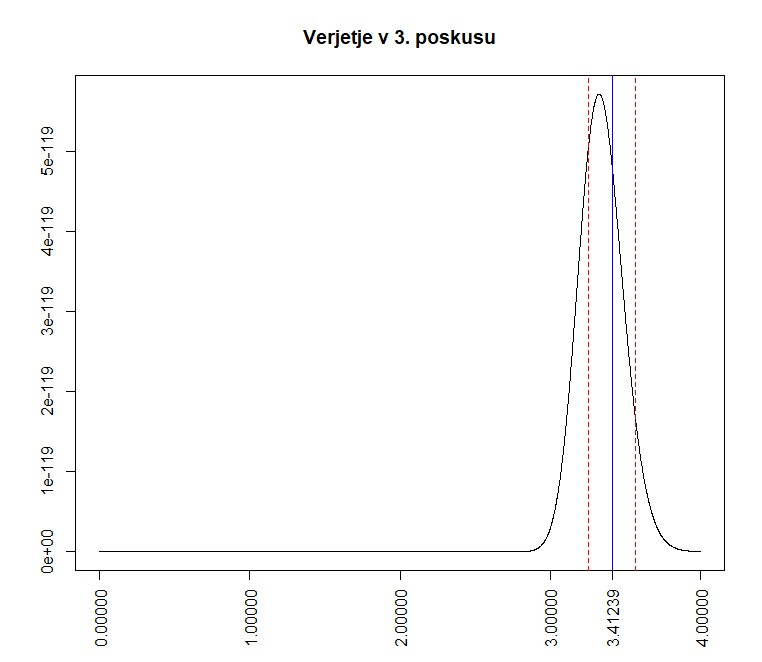
\includegraphics[scale = 0.4]{VerjetjeMM3}
		\caption{Verjetje za oceno cenilke $\theta$, pridobljene po metodi momentov, v tretjem poskusu}
	\end{figure}
	
	Tudi tukaj pridemo do podobnih sklepov, kot v podpoglavju \ref{subsect: 2D} - $SE$-okolica cenilke vsebuje maksimum gostote in je razmeroma majhna zahvaljujoč majhni standardni napaki cenilke. Standardne napake za to cenilko so v resnici presenetljivo blizu vrednostim standardnih napak pri cenilki pridobljeni z metodo največjega verjetja. V primeru, ko napake zaokrožimo na tri decimalke natančno se razlika pojavi samo v zadnjem poskusu, kjer znaša $0{,}01$. To nam pove, da je tudi cenilka, ki smo jo pridobili po metodi momentov, razmeroma dobra alternativa, še posebej zato, ker jo je veliko lažje izračunati.
	
	Dodatno je spodaj ponovno priložen graf na katerem so narisane vse tri gostote, za vizualno primerjavo.
	\begin{figure}[h!]
		\label{fig: 2Eplot4}
		\centering
		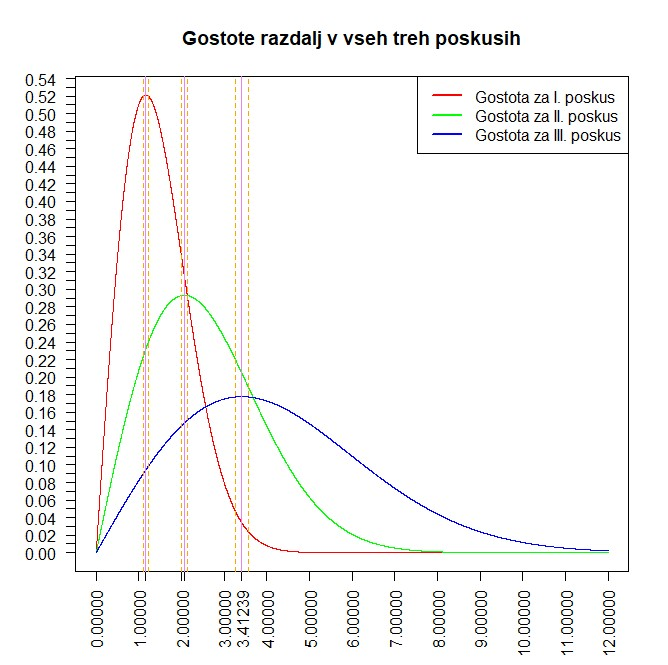
\includegraphics[scale = 0.4]{VerjetjeMM4}
		\caption{Verjetja za vse ocene cenilke $\theta$, pridobljene po metodi momentov}
	\end{figure}
	
	\subsection{Histogram meritev in grafi gostot cenilk} \label{subsect: 2F}
	Da se dokončno prepričamo, da sta izračunani cenilki dobri, bomo za vsak poskus narisali histogram meritev in nanj dorisali gostoti za obe cenilki. Pri določanju širine razredov za histograme bomo uporabili modificirano Freedman-Diaconisovo pravilo, po katerem naj bi širina vsakega razreda bila približno $\frac{2{,}6IQR}{\sqrt[3]{n}}$, kjer je $n$ število podatkov, $IQR$ pa njihov interkvartilni razmik. Skripta \textit{SlucajniSprehodiHIST.R} poračuna te širine za vsak eksperiment ter nato izriše pripadajoče histograme skupaj z gostotama obeh cenilki na vrhu. Skripta te grafe tudi izriše, so pa tudi prikazani spodaj.
	
	\begin{figure}[h!]
		\label{fig: 2FHist1}
		\centering
		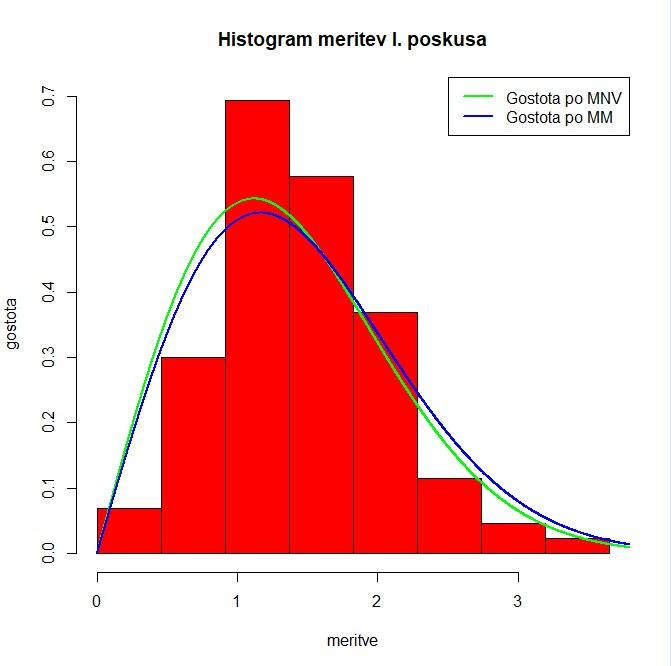
\includegraphics[scale=0.3]{Hist1}
		\caption{Histogram meritev v prvem poskusu skupaj z gostotama za pripadajoči cenilki.}
	\end{figure}

	\begin{figure}[h!]
		\label{fig: 2FHist2}
		\centering
		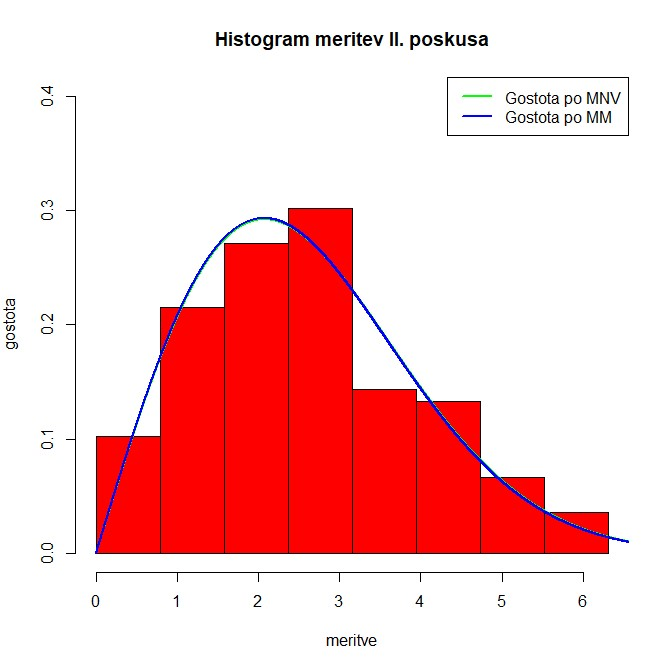
\includegraphics[scale=0.3]{Hist2}
		\caption{Histogram meritev v drugem poskusu skupaj z gostotama za pripadajoči cenilki.}
	\end{figure}	
	
	\begin{figure}[h!]
		\label{fig: 2FHist3}
		\centering
		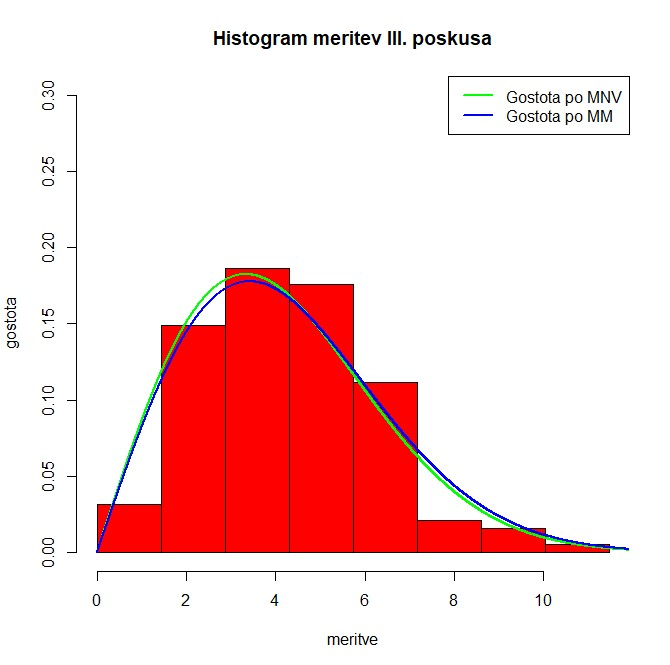
\includegraphics[scale=0.3]{Hist3}
		\caption{Histogram meritev v tretjem poskusu skupaj z gostotama za pripadajoči cenilki.}
	\end{figure}
	
	Vidimo lahko, da se na vsakem grafu obe gostoti medseboj, sicer z manjšimi odstopanji, razmeroma dobro prilegata. V primeru drugega poskusa, se v resnici skoraj popolnoma prekrivata. Tudi s histogrami je podobno - obe gostoti se prilegata obliki, ki jo tvorijo stolpci historgrama. Lahko torej sklepamo, da bi z večanjem vzorcev proti neskončnosti histogram ">konvergiral"< proti grafu gostote. Dokončno torej zatrdimo, da sta obe cenilki res dobri.
	
	\section{Temperature}\label{sect: Temperature}
	V datoteki \textit{Temp\_LJ.csv} imamo podane povprečne mesečne temperature od leta $1986$ do $2020$. Glede na dane podatke bi želeli uporabiti model, ki bo čim bolje napovedal temperature v prihodnosti. 
	Predlagana sta nam dva modela. Model $A$ vključuje linearen trend in sinusno nihanje s periodo enega leta, model $B$ pa vključuje linearen trend in člene, od katerih vsak spreminja temperaturo za svoj mesec. S pomočjo programskega jezika \textbf{R} narišemo graf temperatur v odvisnosti od meseca. Koda za izris tega grafa se nahaja v skripti \textit{Temperature.R}.
	
	\begin{figure}[h!]
		\label{fig: Scatter3}
		\centering
		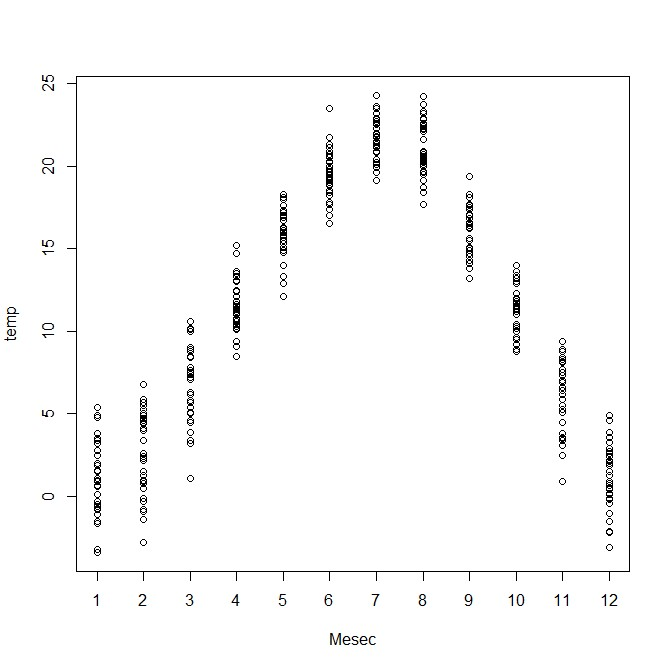
\includegraphics[scale = 0.4]{Scatter3}
		\caption{Razpršen graf povprečnih mesečnih temperatur glede na mesec.}
	\end{figure}

	Opazimo, da se v podatkih res skriva nek trend, zato je seveda smiselno, da premislimo kateri model bi bil za to najbolj primeren. Seveda sta glavna kandidata modela $A$ in $B$. Le ta bosta predmet obravnave v nadaljevanju tega poglavja. V prvem podpoglavju bomo preizkusili model $A$ znotraj modela $B$, v drugem pa bomo poračunali Akaikejevo informacijo za oba modela.
	
	\subsection{Preizkus modela $A$ znotraj modela $B$}\label{susect: 3A}
	Da preizkusimo model $A$ znotraj $B$, najprej zapišimo oba modela. Model $A$ je podan z enačbo $Y = a + bX + c\sin(\frac{X\pi}{6})+ d\cos(\frac{X\pi}{6}) + e$, kjer so $a, b, c~\text{in}~d$ parametri modela, $e$ pa je normalno porazdeljen šum s pričakovano vrednostjo $0$ in varianco $\sigma^2$. Model $B$ je podan z enačbo $Y = m(X) + kx + f$, kjer so $k$ ter $$m(X) = \begin{cases}
		m_1; & X \mod 12 = 1 \\
		m_2; & X \mod 12 = 2 \\
		\vdots & \\
		m_{12}; & X \mod 12 = 0 \\
	\end{cases}$$ parametri modela, $f$ pa je normalno porazdeljen šum s pričakovano vrednostjo $0$ in varianco $\sigma^2$.

	V obeh primerih je $X$ slučajna spremenljivka, ki zavzame vrednosti med $1$ in $420$ (slednje število je enako številu podatkov v \textit{Temp\_LJ.csv}), $Y$ pa je povprečna temperatura za mesec, ki pripada vrednosti $X\mod 12$.
	
	Ker bo v matrični obliki lažje delat, v njo prepišemo oba modela. Od zdaj najprej bo $Y$ vektor velikosti $420$, ki vsebuje temperature iz \textit{Temp\_LJ.csv}, z $e$ označimo normalno porazdeljen vektor šumov $\begin{bmatrix}
		e_1 & e_2 & \cdots & e_{420}
	\end{bmatrix}^{\top}$ (kjer so vsi $e_i$ medseboj neodvisni) za katerega velja, da je $E[e]=0$ in $Var(e) = \sigma^2 I_{420}$. Poleg tega z $\beta$ označimo vektor parametrov modela $\begin{bmatrix}
	a & b & c & d
	\end{bmatrix}^{\top}$.
	
	Matrična oblika modela $A$ je potem $$Y = \begin{bmatrix}
		1 & X_1 & \sin(\frac{X_1\pi}{6}) & \cos(\frac{X_1\pi}{6}) \\
		1 & X_2 & \sin(\frac{X_2\pi}{6}) & \cos(\frac{X_2\pi}{6}) \\
		\vdots & \vdots & \vdots & \vdots \\
		1 & X_{420} & \sin(\frac{X_{420}\pi}{6}) & \cos(\frac{X_{420}\pi}{6}) \\
	\end{bmatrix} \begin{bmatrix}
		a \\
		b \\
		c \\
		d
	\end{bmatrix} + \begin{bmatrix}
		e_1 \\
		e_2 \\
		\vdots \\
		e_{420}
	\end{bmatrix} = X\beta + e$$

	Pri matrični obliki modela $B$ moramo biti malo bolj previdni, saj prosti parameter $m(X)$ v resnici ni samo en parameter, ampak skupek dvanajstih. Naivno bi morda rekli, da se matrični zapis modela glasi $$Y = \begin{bmatrix} 
		1 & X_1 \\
		1 & X_2 \\
		\vdots & \vdots \\
		1 & X_{420}
	\end{bmatrix} \begin{bmatrix}
		m(i) \\
		k
	\end{bmatrix} + f = \bar{X}\bar{\beta} + f$$

	Pri tem $m(i)$ sprejme vrstico, v kateri se nahaja po množenju z matriko $X$ in vrne vrednosti, ki so navedene zgoraj. Ta zapis ni najboljši, saj se izraz močno zakomplicira, prihranimo pa samo nekaj vrstic v zapisu.

	Bolj primerna oblika modela $B$, s katero nam bo seveda tudi lažje delati, je $$Y = \begin{bmatrix}
		1 & 0 & 0 & \cdots & 0 & X_1 \\
		0 & 1 & 0 & \cdots & 0 & X_2 \\
		\vdots & \vdots & \vdots & & \vdots & \vdots \\
		0 & 0 & \cdots & 0 & 1 & X_{12} \\
		1 & 0 & 0 & \cdots & 0 & X_{13} \\
		0 & 1 & 0 & \cdots & 0 & X_{14} \\
		\vdots & \vdots & \vdots & & \vdots & \vdots \\
		0 & 0 & \cdots & 0 & 1 & X_{420}
	\end{bmatrix} \begin{bmatrix}
		m_1 \\
		m_2 \\
		\vdots \\
		m_{12} \\
		k
	\end{bmatrix} + f = \bar{X}\bar{\beta} + f$$
	
	Oblika nazorno pokaže, da so $m_1, \ldots m_{12}$ vsi parametri, ki pa se v modelu pojavijo pod določenimi pogoji (v tem primeru je to, kateri mesec obravnavamo). Omenimo še, da je $f =\begin{bmatrix}
		f_1 & f_2 & \cdots & f_{420}
	\end{bmatrix}^{\top}$, tako kot $e$, normalno porazdeljen vektor šumov s pričakovano vrednostjo $0$ in variančno matriko $\sigma I_{420}$.

	Sedaj, ko imamo v matrični obliki zapisana modela, se lahko lotimo preverjanja modela $A$ znotraj modela $B$. Postopek, ki ga bomo ubrali, je naslednji: Najprej bomo po metodi najmanjših kvadratov poračunali cenilki za $\beta$ in $\bar{\beta}$, nato s pomočjo le teh za vsak model poračunali residuale in preko njih $RSS$. S pomočjo slednjih, bomo izračunali kvocient $F$ in ga primerjali z inverzom kumulativne funkcije Fisherjeve porazdelitve za stopnji tveganja $0{,}01$ in $0{,}05$. Če bo $F \geq F^{-1}_{Fisher(9, 407)}(1 - \alpha)$ za stopnjo tveganja $\alpha$, bomo model $A$ znotraj $B$ zavrnili, sicer pa ga bomo sprejeli.

	\subsubsection{Cenilki $\beta$ in $\bar{\beta}$ po Metodi najmanjših kvadratov}\label{subsubsect: 3ACenilki}
	
	S predavanj vemo, da je cenilka po metodi najmanjših kvadratov za vektor parametrov $\gamma\in\R^p$ v modelu $Y = Z\gamma + \varepsilon$, kjer je $\varepsilon \sim N(0, \sigma^2 I_n)$, enaka $\widehat{\gamma} = (X^{\top}X)^{-1}X^{\top}Y$. Na ta način potem pridobimo cenilki za $\beta$ in $\bar{\beta}$. Pri tem uporabimo \textbf{R} skripto \textit{Temperature.R}, ki ob zagonu v konzolo izpiše cenilki za $\beta$ in $\bar{\beta}$. ti cenilki sta navedeni spodaj.
	
	\[ 
	\widehat{\beta} = \begin{bmatrix}
			10{,}1300627498747 \\
			0{,}00535203760946302 \\                     
			-5{,}10138050301417 \\
			-9{,}04714874745839
		\end{bmatrix}~\text{in}~\widehat{\bar{\beta}} = \begin{bmatrix}
			-0{,}252767273576098 \\
			1{,}45041783380018 \\
			5{,}76503151260504 \\
			10{,}302502334267 \\
			14{,}8685445845005 \\
			18{,}5317296918767 \\
			20{,}5434862278245 \\
			19{,}9838141923436 \\
			14{,}9555707282913 \\
			10{,}2187558356676 \\
			4{,}95051237161531 \\
			0{,}156554621848738 \\
			0{,}00538632119514473
	\end{bmatrix}
	\]
	
	\subsubsection{Residuali in RSS obeh modelov}\label{subsubsect: 3AResiduali}
	Zdaj, ko imamo cenilki za $\beta$ in $\bar{\beta}$ po metodi najmanjših kvadratov lahko poračunamo residuale. V teoretičnem modelu $Y = Z\gamma + \varepsilon$, kot je bil opisan prej v podpodpoglavju \ref{subsubsect: 3ACenilki}, residuale $\widehat{\varepsilon}_i$ poračunamo s formulo $\widehat{\varepsilon}_i = Y_i - \sum_{j = 1}^{p}z_{ij}\widehat{\gamma}_j$, kjer je $\widehat{\gamma}$ cenilka za $\gamma$ po metodi najmanjših kvadratov. Kadar računamo s pomočjo računalnika, je bolj priročen matrični zapis $\widehat{\varepsilon} = Y - Z\widehat{\gamma}$. Količina $RSS$ tega modela je ravno enaka $2$-normi vektorja rezidualov $\widehat{\varepsilon}$ oziroma vsoti $\sum_{i = 1}^{n}\widehat{\varepsilon}_i^2$. Skripta \textit{Temperature.R} izračuna tako reziduale kot $RSS$ za oba modela, a (v konzolo) izpiše samo $RSS$. Vrednosti $RSS$ so tudi navedene v spodnji tabeli
	
	\begin{table}[h!]
		\centering
		\begin{tabular}{| c | c |}
			\hline
			Model & RSS \\ \hline
			$A$ & $35{,}5045981004312$ \\ \hline
			$B$ & $33{,}9190280253558$ \\ \hline
		\end{tabular}
		\caption{Tabela vrednosti $RSS$ za modela $A$ in $B$}
	\end{table}
	
	\subsubsection{Preizkus modela $A$ v $B$ s stopnjama tveganja $0{,}01$ in $0{,}05$}\label{subsubsect: 3APreizkus}
		Končno imamo vse, kar potrebujemo, da preizkusimo model $A$ znotraj $B$. Skripta \textit{Temperature.R} poleg vseh ostalih prej omenjenih vrednosti v konzolo izpiše tudi izračunan $F$. Ta znaša $F = 2{,}1139462554871$. Poleg tega smo poračunali tudi $F_{Fisher(9, 407)}^{-1}(1-\alpha)$ za $\alpha = 0{,}01$ ter $\alpha = 0{,}05$. Vrednosti sta predstavljeni v spodnji tabeli.
		
		\begin{table}[h!]
			\centering
			\begin{tabular}{| c | c | c |}
				\hline
				$\alpha$ & $F_{Fisher(9, 407)}^{-1}(1-\alpha)$ & $F_{Fisher(9, 407)}^{-1}(1-\alpha) <= F$\\ \hline
				$0{,}01$ & $2{,}45105980939293$ & Ne \\ \hline
				$0{,}05$ & $1{,}9028951359083$ & Da \\ \hline
			\end{tabular}
			\caption{Tabela vrednosti $F_{Fisher(9, 407)}^{-1}(1-\alpha)$ za modela $\alpha = 0{,}01$ in $\alpha = 0{,}05$}
		\end{table}
		V tretjem stolpcu so tudi rezultati primerjav $F \geq F_{Fisher(9, 407)}^{-1}(1-\alpha)$. Če neenakost velja, model $A$ znotraj $B$ zavrnemo. To se zgodi ravno pri vrednosti $\alpha = 0{,}05$, ne pa tudi pri $\alpha = 0{,}01$. 
		
	\subsection{Akaikejeva informacija modelov}\label{subsect: 3B}
	Preostane nam samo še izračun Akaikejeve informacije. To bomo storili po formuli $AIC = 2m + n\ln(RSS)$, kjer je $m$ število parametrov, $n$ število podatkov oziroma opažanj ter $RSS$ količina, ki smo jo že poračunali za oba modela. Tudi te vrednosti izračunamo v skripti \textit{Temperature.R} in so avtomatsko izpisane v konzolo. Poleg tega so vrednosti predstavljene tudi v spodnji tabeli.

	\begin{table}[h!]
		\centering
		\begin{tabular}{| c | c |}
			\hline
			Model & $AIC$ \\ \hline
			$A$ & $1507{,}25812906086$ \\ \hline
			$B$ & $1506{,}06998535212$ \\ \hline
		\end{tabular}
		\caption{Tabela vrednosti $AIC$ modelov $A$ in $B$}
	\end{table}
	
	Opazimo, da sta si $AIC$ modelov $A$ in $B$ blizu, kar lahko vidimo tudi na grafu, ki primerja modela s priloženimi podatki. 
	
	\begin{figure}[h!]
		\label{fig: 3BCompare}
		\centering
		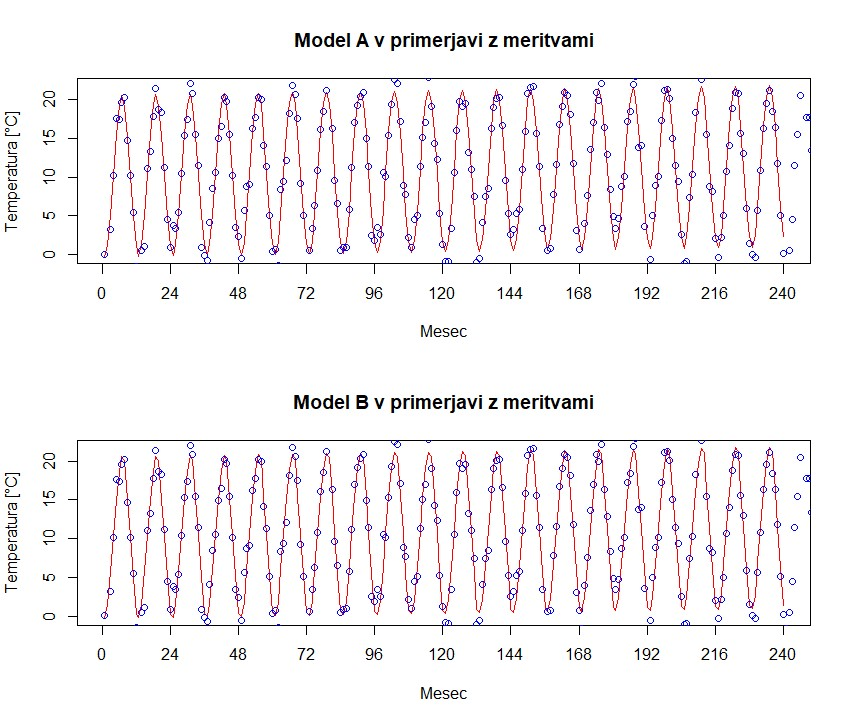
\includegraphics[scale=0.4]{PrimerjavaModelov}
		\caption{Primerjava prileganja modelov A in B s podatki iz \textit{Temp\_LJ.csv}}
	\end{figure}
	
	 Opazimo tudi, da je $AIC(B) \leq AIC(A)$, od koder lahko sklepamo, da je model $B$ boljši od modela $A$.
	
	\begin{thebibliography}{3}
		\bibitem{bib:Rice} J.~Rice, \emph{Mathematical Statistics \& Data Analysis}, 3rd ed., Duxbury, Berkeley, $2007$.
		\bibitem{bib:Rayleigh} \emph{Rayleighjeva porazdelitev}, v: Wikipedia,~Prosta enciklopedija, [ogled 14.~7.~2022], dostopno na \url{https://sl.wikipedia.org/wiki/Rayleighjeva_porazdelitev}.
	\end{thebibliography}
\end{document}